\chapter{状態方程式、放射、真空エネルギー}

\lectureoverview{一様な宇宙の歴史は、主としてそのスケール因子\(a(t)\)の歴史である。フリードマン方程式は幾何学を与えるが、物質の状態方程式は、空間が膨張する間にエネルギー密度がどのように変化するかを教えてくれる。まず流体がする仕事から\(\rho\propto a^{-3(1+w)}\)を導き、次に光子の運動量移動を数えることによって放射に対する\(P=\rho/3\)を得て、最後に\(P=-\rho\)によって真空エネルギーを同定する。正の真空エネルギーはド・ジッター膨張を生み、曲率と宇宙定数の符号は、単純な力学系として読むことのできるバウンス解と再収縮解を生む。}

\section{スケール因子と欠けている物質の法則}

まず、どこへ向かっているのかを確認しよう。一様等方近似の下では、主要な宇宙論的歴史は一つの関数\(a(t)\)に符号化されている。その関数を知ることは宇宙についてのすべての問いに答えるわけではないが、距離、膨張率、そして大規模な時代の順序を決定する。この講義の目的は、まだそれらの時代を観測的に確立することではない。モデルを可能にする状態方程式を、基礎物理学から導くことである。

二つの基準モデルがすでに現れている。
\begin{equation}
a(t)\propto t^{2/3}
\qquad\text{(matter domination)},
\end{equation}
および
\begin{equation}
a(t)\propto t^{1/2}
\qquad\text{(radiation domination)}.
\end{equation}
どちらの法則もすべての時間に対して厳密ではない。放射は有用な初期時間の近似を与え、物質はその後の中期の近似を与える。真空エネルギーは最終的に後期の振る舞いを再び変える。当面の問いは、観測がこれらの時代をどのように明らかにするかではなく、フリードマン方程式の対応する右辺を何が区別するかである。

\begin{figure}[htbp]
\centering
\includegraphics[width=0.72\textwidth]{lecture_05_figure_02.png}
\caption{復習したスケール因子の冪則と、新たに導入された密度の記号。これは完成した導出ではなく、過渡的な板書状態である。}
\label{fig:c05-review-board}
\lectureframe{00:03:18.380}
\end{figure}

欠けている橋渡しは状態方程式である。それは、フリードマン方程式の右辺のエネルギー密度がスケール因子とともにどのように変化するかを決定する。二つの基準法則は
\begin{equation}
\rho_{\text{matter}}=\frac{\rho_0}{a^3},
\qquad
\rho_{\text{rad}}=\frac{\rho_0}{a^4}.
\label{eq:c05-benchmark-densities}
\end{equation}
である。物質は体積とともに薄まり、体積は\(a^3\)としてスケールする。放射はさらに\(a\)の1乗分だけ余分に減少する。両方の規則を、圧力とエネルギー密度の関係の帰結として理解したい。

\section{圧力から密度スケーリング則へ}

状態方程式は一般に密度、圧力、温度、その他の変数を含みうる。ここで考える宇宙論的成分に対しては、有用な定数\(w\)の形
\begin{equation}
P=w\rho,
\label{eq:c05-eos}
\end{equation}
を採用する。ここで\(w\)は流体を特徴づける。板書では大文字の\(W\)が用いられているが、我々は慣例的な小文字の\(w\)を用いる。この線形な形は以下の重要な場合を覆うが、あらゆる可能な流体が従う法則ではなく、単純化したアンザッツである。

非相対論的物質では、エネルギー密度は静止エネルギーによって支配される。\(n\)を数密度、\(m\)を粒子質量とすると、概略
\begin{equation}
\rho\simeq nmc^2.
\end{equation}
となる。因子\(c^2\)は、小さな静止質量さえも巨大なエネルギーの貯蔵庫にする。塵の粒を完全に消滅させれば、巨視的な量のエネルギーが解放されるであろう。これに対して圧力は、粒子が壁に衝突するときの運動量移動によって生じ、\(nmv^2\)の程度である。ボウリングの球はピンポン球よりも多くの運動量を移動させるが、冷たい気体ではすべての関連する速度が\(v\ll c\)を満たす。したがって
\begin{equation}
\frac{P}{\rho}\sim\frac{v^2}{c^2}\ll1,
\qquad
w\simeq0.
\label{eq:c05-dust-eos}
\end{equation}
となる。放射は\(c\)で運動するので、この近似を共有しない。我々はその\(w\)の値を仮定するのではなく導出する。

次に、状態方程式~\eqref{eq:c05-eos}を\(\rho\)のスケーリング則に変える一般的な仕組みが必要である。実験室の箱で十分である。銀河を文字通り箱に入れることはできないが、粗視化した後ではそれらは粒子のように振る舞い、エネルギーと圧力の関係は局所的に導出できる。

\begin{figure}[htbp]
\centering
\includegraphics[width=0.86\textwidth]{lecture_05_figure_03.png}
\caption{状態方程式、復習した密度スケーリング、そして熱力学の箱が一つの板書にある。講師が以前の書き込みの一部を隠しているため、この画像は完全な転記ではなく、レイアウトと可視の方程式のために用いる。}
\label{fig:c05-box-board}
\lectureframe{00:13:39.612}
\end{figure}

板書の左側には復習した宇宙論的スケーリングがあり、右側では箱の議論が始まる。合わせて読むと、可視の内容は
\begin{equation}
\rho_{\text{matter}}=\frac{\rho_0}{a^3},
\qquad
\rho_{\text{rad}}=\frac{\rho_0}{a^4},
\qquad
P=w\rho.
\end{equation}
を結びつけている。我々の課題は、状態方程式から二つの密度法則を導出することである。

一方の壁の面積は\(A\)である。これを外側へ\(dx\)だけ動かすと、
\begin{equation}
dV=A\,dx.
\end{equation}
圧力は単位面積あたりの力であるから、壁に働く力は\(PA\)である。気体は仕事\(PA\,dx=P\,dV\)を行い、内部に残るエネルギーは減少する。
\begin{equation}
dE=-P\,dV.
\label{eq:c05-work-law}
\end{equation}
\begin{figure}[htbp]
\centering
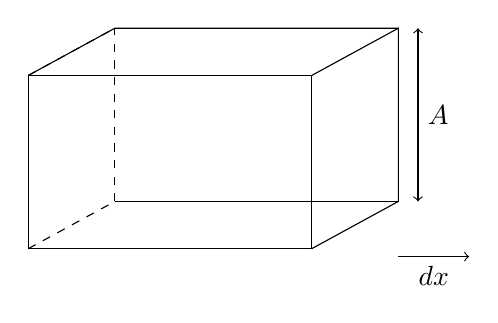
\begin{tikzpicture}[scale=1.0]
\draw (0,0) -- (3.6,0) -- (3.6,2.2) -- (0,2.2) -- cycle;
\draw (3.6,0) -- (4.7,0.6) -- (4.7,2.8) -- (3.6,2.2);
\draw (0,2.2) -- (1.1,2.8) -- (4.7,2.8);
\draw (1.1,0.6) -- (4.7,0.6);
\draw[dashed] (0,0) -- (1.1,0.6);
\draw[dashed] (0,2.2) -- (1.1,2.8);
\draw[dashed] (1.1,0.6) -- (1.1,2.8);
\draw[<->] (4.95,0.6) -- (4.95,2.8);
\node[right] at (4.95,1.7) {\(A\)};
\draw[->] (4.7,-0.1) -- (5.6,-0.1);
\node[below] at (5.15,-0.1) {\(dx\)};
\end{tikzpicture}
\caption{面の面積\(A\)と変位\(dx\)をもつ熱力学の箱の明快な再構成。}
\label{fig:c05-box-redraw}
\end{figure}

全エネルギーは
\begin{equation}
E=\rho V.
\end{equation}
である。微分すると
\begin{equation}
d(\rho V)=\rho\,dV+V\,d\rho.
\end{equation}
が得られる。式~\eqref{eq:c05-work-law}に代入すると
\begin{equation}
\rho\,dV+V\,d\rho=-P\,dV.
\end{equation}
となる。\(P=w\rho\)を代入すると、
\begin{equation}
V\,d\rho=-(1+w)\rho\,dV.
\end{equation}
この結果は有用な式への準備段階であり、まだそこには達していない。\(\rho V\)で割ると、
\begin{equation}
\frac{d\rho}{\rho}=-(1+w)\frac{dV}{V}.
\end{equation}
\begin{figure}[htbp]
\centering
\includegraphics[width=0.78\textwidth]{lecture_05_figure_04.png}
\caption{分離された密度・体積の式と対数積分の始まり。右辺全体は、隠れたピクセルからではなく、先行する代数から再構成される。}
\label{fig:c05-log-board}
\lectureframe{00:15:35.600}
\end{figure}

画面には分離された式とその始まり\(\log\rho=\)が示されている。積分を直接完成させると、
\begin{equation}
d(\log\rho)=-(1+w)\,d(\log V),
\end{equation}
したがって
\begin{equation}
\log\rho=-(1+w)\log V+\text{const.}
\end{equation}
指数をとると、
\begin{equation}
\rho\propto V^{-(1+w)}.
\end{equation}
これが密度・体積の法則である。

ここで箱から宇宙論に戻る。壁を一つだけ動かしたのは便利な導出であって、異方性を仮定したわけではない。三つの方向すべてを一様に膨張させても同じ仕事の関係が得られ、共動体積は
\begin{equation}
V\propto a^3.
\end{equation}
のようにスケールする。したがって
\begin{equation}
\boxed{\rho\propto a^{-3(1+w)}}.
\label{eq:c05-density-scaling}
\end{equation}
\(d\)次元空間では指数\(3\)は\(d\)になるであろうが、議論の残りの部分は変わらない。

\section{最初の応用：物質と放射}

これで、復習の式を仮定ではなく帰結として再現できる。

非相対論的物質については
\begin{equation}
w=0.
\end{equation}
ととる。すると
\begin{equation}
\rho\propto a^{-3},
\end{equation}
となり、これはまさに物質の希薄化の法則である。

放射については、暫定的に
\begin{equation}
w=\frac13.
\end{equation}
ととる。これが正しければ、
\begin{equation}
\rho\propto a^{-3(1+1/3)}=a^{-4}.
\end{equation}
となる。したがって余分な逆べきは\(w=1/3\)と等価である。未解決の段階は、その値を光子の物理から導出することである。

\section{なぜ放射圧はそのエネルギー密度の三分の一なのか}

放射は電磁波としても、質量のない粒子としても記述できる。光子を用いて、箱の中の光子気体の圧力を計算する。箱は二次元で描かれているが、気体とその角度分布は三次元である。光子は光速で運動し、暫定的な壁で弾性的に跳ね返る。

当面、すべての光子が同じエネルギー\(\epsilon\)をもつと仮定する。この単純化は、異なるエネルギーの寄与を加えるときに消える。\(\vec{\pi}\)を光子の運動量ベクトルとする。通常の\(p\)は、\(P\)がすでに圧力を表すため避ける。質量のない粒子は次の関係を満たす。
\begin{equation}
\epsilon=c\,\pi,
\end{equation}
ここで\(\pi=|\vec{\pi}|\)である。講義で用いる単位では\(c=1\)なので、
\begin{equation}
\epsilon=\pi.
\end{equation}
\(\nu\)を光子数密度とすると、エネルギー密度は
\begin{equation}
\rho=\epsilon\,\nu.
\end{equation}
である。\(x\)軸を一方の壁に垂直にとる。短い時間間隔\(\Delta t\)の間に、その法線と角度\(\theta\)をなして運動する光子が壁に到達するのは、厚さ
\begin{equation}
\Delta x=\Delta t\cos\theta.
\end{equation}
のスラブ内から出発した場合だけである。反射すると、その運動量の\(x\)成分の符号が反転するので、壁に移される運動量は
\begin{equation}
\Delta \pi_x=2\epsilon\cos\theta.
\end{equation}
である。力は単位時間あたりの運動量移動であるから、一回の衝突は\(\Delta \pi_x/\Delta t\)だけ寄与する。スラブ内の光子の数は\(\nu A\Delta x\)であるが、そのうち壁に向かって運動するのは半分だけなので、関係する数は\(\tfrac12 \nu A\Delta x\)である。全力を壁の面積\(A\)で割ると、
\begin{align}
P(\theta)
&=
\frac{1}{A}
\left(\frac{2\epsilon\cos\theta}{\Delta t}\right)
\left(\frac12 \nu A\Delta x\right) \\
&=
\epsilon\nu\cos\theta\frac{\Delta x}{\Delta t} \\
&=
\epsilon\nu\cos^2\theta \\
&=
\rho\cos^2\theta.
\end{align}
が得られる。この結果が角度に依存するのは、それが一方向に進む光子からの寄与にすぎないからである。

\begin{figure}[htbp]
\centering
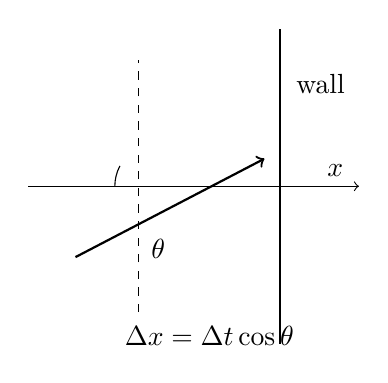
\begin{tikzpicture}[scale=1.0]
\draw[thick] (0,0) -- (0,4);
\draw[->] (-3.2,2) -- (1.0,2);
\node[above] at (0.7,2) {\(x\)};
\draw[dashed] (-1.8,0.4) -- (-1.8,3.6);
\node[below] at (-0.9,0.35) {\(\Delta x=\Delta t\cos\theta\)};
\draw[->,thick] (-2.6,1.1) -- (-0.2,2.35);
\node[below] at (-1.55,1.45) {\(\theta\)};
\draw (-2.1,2) arc[start angle=180,end angle=152,radius=0.55];
\node[right] at (0.08,3.3) {wall};
\end{tikzpicture}
\caption{角度\(\theta\)で壁に入射する光子の運動量。放射圧を導出するために用いた幾何。}
\label{fig:c05-photon-pressure}
\end{figure}

等方的な分布について平均する。\(\mathbf n=(n_x,n_y,n_z)\)を光子の方向に沿った単位ベクトルとする。すると
\begin{equation}
n_x=\cos\theta,
\qquad
n_x^2+n_y^2+n_z^2=1.
\end{equation}
等方的な気体では、\(n_x^2\)、\(n_y^2\)、\(n_z^2\)の平均は等しい。上の恒等式を平均すると、
\begin{equation}
\langle n_x^2\rangle+\langle n_y^2\rangle+\langle n_z^2\rangle=1,
\end{equation}
となり、対称性により各項は同じなので、
\begin{equation}
\langle n_x^2\rangle=\langle \cos^2\theta\rangle=\frac13.
\end{equation}
したがって
\begin{equation}
P=\rho\langle \cos^2\theta\rangle=\frac{\rho}{3}.
\end{equation}
よって放射の状態方程式は
\begin{equation}
P=\frac13\rho,
\qquad
w=\frac13.
\end{equation}
である。因子\(1/3\)は、単位ベクトルの二乗を分け合う空間方向の数である。\(d\)個の等方的な空間次元では、同じ議論から\(\langle n_x^2\rangle=1/d\)が得られるであろう。これで、冒頭で約束した微視的導出が完了する。

\subsection{放射の議論を試す問い}

\begin{classroomqa}
\audiencequestion{すべての光子が同じエネルギーをもつ必要があるのだろうか。}
\lecturerresponse{いいえ。各エネルギー区間で別々に計算すればよい。各区間は自身のエネルギー密度の三分の一に等しい圧力に寄与するので、スペクトル全体で和をとっても\(P=\rho/3\)が保たれる。等エネルギーという仮定は、記法を短く保つためだけのものであった。\lecturetimestamp{00:39:08--00:39:36}}
\end{classroomqa}

\begin{classroomqa}
\audiencequestion{吸収する黒い壁は完全な鏡と同じ答えを与えるだろうか、また空っぽの空間における壁とは何か。}
\lecturerresponse{熱平衡にある黒い壁は放射を吸収し再放出し、同じ平均の運動量の釣り合いを生じる。宇宙空間には文字どおりの壁はなく、その面は想像上の境界である。外へ向かって横切るすべての光子に対して、等方性により内向きの平均的な補償流が供給されるので、局所的な運動量流の計算は変わらない。教室の放射は主として熱的な宇宙マイクロ波背景放射であり、この平衡の描像はそれに対してとりわけ自然である。\lecturetimestamp{00:39:37--00:41:19}}
\end{classroomqa}

\begin{classroomqa}
\audiencequestion{量子統計は\(P=\rho/3\)を変えるのだろうか。}
\lecturerresponse{いいえ。ボース統計は、光子が利用可能なモードをどのように占有するかを決め、したがってスペクトルと全\(\rho\)を決めるが、質量のない粒子の等方的な応力は、そのエネルギー密度の三分の一のままである。\lecturetimestamp{00:41:51--00:42:02}}
\end{classroomqa}

\begin{classroomqa}
\audiencequestion{光子が互いに散乱する場合はどうか。}
\lecturerresponse{通常の光子-光子散乱は極めて弱いので、ここでのその補正は無視できる。十分に高い温度と密度では、衝突が電子-陽電子対を生成し、有効な粒子の内容と状態方程式を変えうる。それは実在の効果であるが、この議論で用いた領域よりはるかに高温の領域に属する。\lecturetimestamp{00:42:02--00:43:08}}
\end{classroomqa}

\begin{classroomqa}
\audiencequestion{壁の面積\(A\)はどうなったのか。}
\lecturerresponse{中間の積は、1個の光子による力に壁に当たる個数を掛けたものであり、その個数は\(A\)に比例する。圧力は力を面積で割ったものなので、最後の割り算で\(A\)が相殺される。中間の表式を早まって圧力と呼んだことが板書の省略であり、力から圧力への段階を復元すれば修正される。\lecturetimestamp{00:43:11--00:44:01}}
\end{classroomqa}

\section{負の圧力と張力の意味}

これまでは、粒子が壁に当たって壁を外へ押していた。その描像は自然に正の圧力を生じるが、可能性を尽くすものではない。

\begin{classroomqa}
\audiencequestion{エネルギー密度自体が負になりうるだろうか。}
\lecturerresponse{量子論は限られた状況で負のエネルギー密度を許し、宇宙定数は形式的にはどちらの符号もとりうる。そのような場合は注意を要し、当面の出発点ではない。よりなじみ深い入口は負の\emph{圧力}であり、これはエネルギー密度が正のままで生じうる。\lecturetimestamp{00:44:25--00:44:59}}
\end{classroomqa}

\begin{classroomqa}
\audiencequestion{圧力はどのようにして負になりうるのか。}
\lecturerresponse{1次元の世界では、箱は線分である。自由に運動する粒子はその両端で跳ね返り、外へ押して正の圧力を与える。代わりに両端を引き伸ばした弦やばねでつなぐ。両端を引き離すと、ばねは両端を内側へ引く。この内向きの力が張力であり、負の圧力の1次元模型である。\lecturetimestamp{00:45:04--00:46:31}}
\end{classroomqa}

\begin{figure}[htbp]
\centering
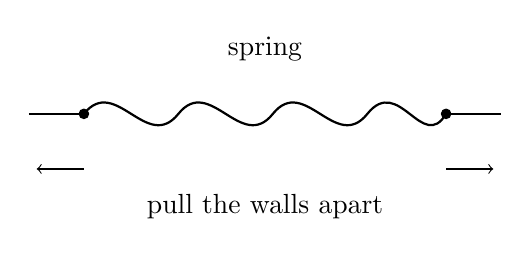
\begin{tikzpicture}[scale=1.0]
\draw[thick] (-3,0) -- (-2.3,0);
\draw[thick] (2.3,0) -- (3,0);
\draw[fill] (-2.3,0) circle (0.06);
\draw[fill] (2.3,0) circle (0.06);
\draw[thick] (-2.3,0)
.. controls (-1.9,0.5) and (-1.5,-0.5) .. (-1.1,0)
.. controls (-0.7,0.5) and (-0.3,-0.5) .. (0.1,0)
.. controls (0.5,0.5) and (0.9,-0.5) .. (1.3,0)
.. controls (1.7,0.5) and (2.0,-0.5) .. (2.3,0);
\draw[->] (-2.3,-0.7) -- (-2.9,-0.7);
\draw[->] (2.3,-0.7) -- (2.9,-0.7);
\node[below] at (0,-0.9) {pull the walls apart};
\node[above] at (0,0.55) {spring};
\end{tikzpicture}
\caption{負の圧力の類推としての1次元のばね。}
\label{fig:c05-tension}
\end{figure}

仕事の収支はそれに応じて逆転する。膨張は正の圧力の気体に仕事をさせ、内部エネルギーを失わせる。張力に逆らって外へ引くと、エネルギーがばねに蓄えられる。より一般には、引力を及ぼす構成要素が互いを、そして境界を内側へ引くことができる。したがって系は\(\rho>0\)かつ\(P<0\)をもち、\(w<0\)となっても矛盾はない。この可能性が中心的なのは、真空のエネルギーがまさにその符号のパターンをもつからである。

\section{真空のエネルギーと宇宙定数}

真空のエネルギーは、空っぽの空間そのものに割り当てられる。量子場の理論は、場のモードに対応する調和振動子の零点運動を通じてそれを動機づけるが、その巨視的な記述のために、この微視的な問題を解く必要はない。定義的な性質は、空っぽの空間が、どこであれ、どれほど大きな領域を選ぼうとも、同じエネルギー密度をもつことである。
\begin{equation}
\rho=\rho_0=\text{const.}
\label{eq:c05-vacuum-density}
\end{equation}
体積\(V\)の領域が真空のエネルギーだけを含むなら、その領域の全エネルギーは
\begin{equation}
E=\rho_0 V.
\end{equation}
\begin{classroomqa}
\audiencequestion{箱は、許される場のモードを制限することによって真空の密度を変えるのだろうか。}
\lecturerresponse{有限領域の全エネルギーが全空間のエネルギーより小さいのは、その領域の体積がより小さいからであり、バルクの密度\(\rho_0\)は同じままである。実際の境界はモードのエネルギーを変え、カシミール効果を生じうるが、その補正が重要になるのは、間隔が関係する波長と同程度である場合である。それは宇宙論で用いられる大規模な真空の密度ではない。 \lecturetimestamp{00:50:06--00:51:25}}
\end{classroomqa}

導入する
\begin{equation}
\Lambda=\frac{8\pi G}{3}\rho_0.
\label{eq:c05-lambda-definition}
\end{equation}
この定義は、フリードマン方程式に現れる組み合わせを吸収している。逆の関係は
\begin{equation}
\rho_0=\frac{3\Lambda}{8\pi G}.
\end{equation}
パラメータ\(\Lambda\)は宇宙定数である。後期の加速を駆動する、正でほぼ一定の成分は、一般にダークエネルギーと呼ばれる。

スケール因子依存性はすでに確定しているので、箱の議論を逆にたどってその圧力を導こう。\(d\rho_0=0\)であるから、
\begin{equation}
dE=d(\rho_0V)=\rho_0\,dV.
\end{equation}
一方、熱力学的な仕事の関係は依然として
\begin{equation}
dE=-P\,dV.
\end{equation}
\(P=w\rho_0\)と書くなら、
\begin{equation}
dE=-w\rho_0\,dV.
\end{equation}
比較により
\begin{equation}
w=-1.
\end{equation}
したがって
\begin{equation}
P=-\rho.
\end{equation}
ばねの類推は、この符号を準備していたのである。正の真空のエネルギーは負の圧力をもち、負の真空のエネルギーは正の圧力をもつ。\(w\)の天文学的測定は、後期の成分が本当に希釈されない真空として振る舞うかどうかを問う。\(w\)が\(-1\)に近いほど、その振る舞いは式~\eqref{eq:c05-vacuum-density}に近づく。

\begin{classroomqa}
\audiencequestion{\(P=-\rho\)は空の宇宙の状態方程式なのか、そして\(\rho_0\)を計算できるのか。}
\lecturerresponse{それは、真空のエネルギーが存在するときの空っぽの空間の状態方程式である。その大きさははるかに難しい。あらゆる量子場とあらゆるエネルギースケールが寄与しうる。まだ発見されていない場も含まれるので、観測値を説明する受け入れられた計算は存在しない。主な難問は、\(w=-1\)をどのように書くかではなく、なぜ正味の\(\rho_0\)がこれほど並外れて小さいのかである。 \lecturetimestamp{00:57:27--00:58:29}}
\end{classroomqa}

\section{フリードマン力学における真空のエネルギー}

以前に純粋な物質と純粋な放射を分離したのと同じように、真空のエネルギーを分離する。\(\rho=\rho_0\)とすると、フリードマン方程式は
\begin{equation}
\left(\frac{\dot a}{a}\right)^2=\Lambda-\frac{k}{a^2},
\label{eq:c05-vacuum-friedmann}
\end{equation}
となり、球面空間、平坦空間、双曲空間に対して\(k=+1,0,-1\)である。正と負の\(\Lambda\)が、\(k\)の3つの選択と組み合わさって6つの符号の場合を与えるが、すべての場合が実解を許すわけではない。

\begin{remark}
講義では\(\Lambda=(8\pi G/3)\rho_0\)を定義しているので、ここでの\(\Lambda\)は\(H^2\)の次元をもつ。一般的な慣習\(G_{\mu\nu}+\Lambda_{\mathrm E}g_{\mu\nu}=8\pi G T_{\mu\nu}\)では、対応するパラメータは\(\Lambda_{\mathrm E}=3\Lambda\)である。
\end{remark}

\subsection{平坦なド・ジッター膨張}

\(k=0\)とおく。すると
\begin{equation}
\left(\frac{\dot a}{a}\right)^2=\Lambda.
\end{equation}
\(\Lambda>0\)に対して、膨張する枝を選ぶ。
\begin{equation}
\dot a=\sqrt{\Lambda}\,a,
\end{equation}
したがって
\begin{equation}
a(t)=C\,e^{\sqrt{\Lambda}\,t}.
\end{equation}
ハッブルパラメータはそのとき一定である。
\begin{equation}
H=\frac{\dot a}{a}=\sqrt{\Lambda}.
\end{equation}
これは平坦スライシングにおけるド・ジッター空間であり、アインシュタインが1917年にその項を導入した直後に宇宙定数解を見出したウィレム・ド・ジッターにちなんで名づけられている。\(\Lambda<0\)で\(k=0\)ならば、\(H^2\)は負になりえないので、式~\eqref{eq:c05-vacuum-friedmann}は実解をもたない。

\begin{classroomqa}
\audiencequestion{ここでハッブルパラメータは本当に一定なのか、そしてこの時空はビッグバンをもつのか。}
\lecturerresponse{純粋な平坦スライシング解では、\(H=\sqrt{\Lambda}\)は厳密に一定である。\(a(t)\to0\)は\(t\to-\infty\)のときのみであるが、この座標パッチは測地線的に完備ではない。過去向きの軌道のいくつかは、有限の固有時間でその境界に到達する。したがって、この式だけでは大域的なビッグバンの問題を決着させない。完全なド・ジッター幾何はこの平坦パッチ以上のものを含んでおり、その点は幾何を詳しく調べるまで保留される。 \lecturetimestamp{01:06:54--01:08:07}}
\end{classroomqa}

物質、放射、曲率、真空のエネルギーを含む宇宙に対する模式的なフリードマン方程式は
\begin{equation}
\left(\frac{\dot a}{a}\right)^2
=
\Lambda+\frac{C_m}{a^3}+\frac{C_r}{a^4}-\frac{k}{a^2}.
\label{eq:c05-mixed-friedmann}
\end{equation}
初期には、\(a\)が小さいとき、逆べき乗の項が支配的で、真空のエネルギーは無視できる。後期には、\(a\)が大きいとき、定数項\(\Lambda\)が支配的である。したがって宇宙は転移を起こす。初期には物質支配または放射支配のように見え、後期にはド・ジッター的な振る舞いに近づく。

指数関数では\(\ddot a>0\)であるため、真空支配は加速膨張となる。遷移の間、加速は厳密に指数関数的である必要はない。物質が依然として方程式~\eqref{eq:c05-mixed-friedmann}に寄与するからである。講義当時の観測は、すでに純粋なド・ジッター期にあるのではなく、この競合の最中に宇宙を捉えたものとして記述されている。

\section{真空エネルギーに関する疑問}

\begin{classroomqa}
\audiencequestion{真空エネルギーが基底状態のエネルギーならば、なぜ負になり得るのか。}
\lecturerresponse{ボソンの振動モードは\(+\tfrac12\hbar\omega\)に寄与するのに対し、フェルミオン的モードは反対の符号で寄与する。正味の真空エネルギーは多数の場とスケールにわたる和であるため、総量が判明する前にはどちらの符号も可能である。寄与が存在すること自体は自然であり、その極めて小さな残差を説明することが難しい部分である。\lecturetimestamp{01:12:00--01:14:12}}
\end{classroomqa}

\begin{classroomqa}
\audiencequestion{一定の\(w=-1\)は将来のビッグリップを意味するのか。}
\lecturerresponse{いいえ。\(w=-1\)の宇宙定数はド・ジッター的な指数関数的膨張を与えるが、ビッグリップと呼ばれる有限時間での発散を生じさせるものではない。そのシナリオは\(w<-1\)の仮説上のファントム成分に属し、それでは宇宙の膨張に伴って密度が増大する。ここではそのような成分は仮定されていない。\lecturetimestamp{01:14:13--01:15:50}}
\end{classroomqa}

\begin{classroomqa}
\audiencequestion{厳密な超対称性があれば真空エネルギーは消えるのか。}
\lecturerresponse{すべてのボソン的自由度がフェルミオン的自由度と対をなすため、零点寄与を相殺し得る。しかし自然界は低エネルギーでの厳密な超対称性を示さない。観測されるボソンとフェルミオンは質量が縮退したパートナーではない。したがって厳密な相殺は、現在観測されている世界における真空エネルギーを説明しない。\lecturetimestamp{01:15:51--01:16:20}}
\end{classroomqa}

\begin{classroomqa}
\audiencequestion{自然な真空エネルギーの推定値と観測値の間の途方もない不一致とは何か。}
\lecturerresponse{普遍定数\(c\)、\(\hbar\)、\(G\)はプランク単位を定義する。速さ\(c\)はあらゆる信号を制限し、\(\hbar\)は普遍的な量子不確定性のスケールを定め、\(G\)はすべてのエネルギーを重力に結合させる。これらから、およそ\(10^{-5}\)グラムのプランク質量と、およそ\(10^{-33}\)センチメートルのプランク長が構成され、したがって、およそプランク長の三乗あたり1プランクエネルギーというプランクエネルギー密度が得られる。これらの単位では、観測された真空密度は講義でおよそ\(10^{-123}\)と述べられており、正確な指数は規約に依存する。謎は、自然に遥かに大きなスケールを示唆する寄与が、なぜこれほど小さな非零の結果を残すのかということである。\lecturetimestamp{01:16:21--01:23:12}}
\end{classroomqa}

\begin{classroomqa}
\audiencequestion{真空からの寄与が予想されるならば、なぜ物理学者は非零の宇宙定数の発見に驚いたのか。}
\lecturerresponse{繰り返される観測の改良は、ゼロと整合する結果を見出し続けていた。その歴史が、未知の厳密な原理、おそらく将来の量子重力理論におけるそれによって完全な相殺が強制されるという心理的期待を促した。最終的な検出はその期待を覆した。驚きは、真空エネルギーが消えなければならないという導出ではなく、数十年にわたるますます厳しいヌル結果を反映していた。\lecturetimestamp{01:23:14--01:26:05}}
\end{classroomqa}

\begin{classroomqa}
\audiencequestion{観測によって暗黒エネルギーが時間とともに変化するかどうかを決定できるか。}
\lecturerresponse{遠い未来における急激な変化を排除することはできないが、数十億年にわたる最近の膨張史を比較することはできる。\(w\)、より一般には\(w(a)\)を測定することは、その期間に密度が進化したかどうかを検証する。講義は当時の制約をおよそ10パーセントの水準でのみ報告している。その数値は歴史的なものであるが、永続する要点は\(w=-1\)が変化しない密度に対応するということである。\lecturetimestamp{01:26:06--01:27:16}}
\end{classroomqa}

\begin{classroomqa}
\audiencequestion{空間次元の数が異なれば結果は違って見えるか。}
\lecturerresponse{全体的な構造は保たれる。\(d\)個の等方な空間次元では、放射は\(w=1/d\)を持ち\(a^{-(d+1)}\)として希薄化するが、ローレンツ不変な真空エネルギーは依然として\(w=-1\)を持つ。フリードマン方程式の数値係数は次元によって変わるが、希薄化する物質、放射、および希薄化しない真空の区別は生き残る。\lecturetimestamp{01:27:16--01:27:57}}
\end{classroomqa}

\section{曲率と力学的類推}

\subsection{正の真空エネルギーを伴う正の曲率}

\(k=+1\) と \(\Lambda>0\) を取る：
\begin{equation}
\left(\frac{\dot a}{a}\right)^2=\Lambda-\frac{1}{a^2}.
\label{eq:c05-closed-vacuum}
\end{equation}
\(a^2\) を掛けると、
\begin{equation}
\dot a^2-\Lambda a^2=-1.
\label{eq:c05-inverted-oscillator}
\end{equation}
\(a\) を仮想粒子の座標とみなす。すると \(\dot a^2\) はその運動項であり、\(-\Lambda a^2\) は上下逆さまの二次ポテンシャルであり、全エネルギーは \(-1\) である。物理的に許される枝は \(a\geq\Lambda^{-1/2}\) をもつ：宇宙は大きなサイズから収縮し、最小で静止に達し、再び膨張する。

厳密解は
\begin{equation}
a(t)=\Lambda^{-1/2}\cosh(\sqrt{\Lambda}\,t).
\label{eq:c05-closed-desitter}
\end{equation}
\begin{equation}
\cosh(\sqrt{\Lambda}\,t)
=
\frac12\left(e^{\sqrt{\Lambda}\,t}+e^{-\sqrt{\Lambda}\,t}\right),
\end{equation} を用いる。
この関数は時間に関して対称である。\(t=0\) では \(a=\Lambda^{-1/2}\) であり、どちらの時間方向に向かっても指数関数的に増大する。したがって閉じたスライシングは、収縮、非特異な最小、再膨張を示す。それは平坦な指数関数的スライシングとは大域的に異なって見えるが、両方の座標系は同じド・ジッター幾何の一部を覆っている。

\subsection{負の宇宙定数}

\(\Lambda=-|\Lambda|\) と書く。もし \(k=+1\) ならば、方程式~\eqref{eq:c05-vacuum-friedmann} はすべての \(a\) に対して負の右辺をもち、一方 \(H^2\geq0\) である。この純粋真空型の実の FRW 解は存在しない。

\(k=-1\) に対して、
\begin{equation}
\left(\frac{\dot a}{a}\right)^2=-|\Lambda|+\frac{1}{a^2}.
\end{equation}
\(a^2\) を全体に掛けると、
\begin{equation}
\dot a^2+|\Lambda|a^2=1.
\label{eq:c05-negative-lambda-oscillator}
\end{equation}
これは調和振動子のエネルギー方程式である。\(a\geq0\) なので、物理的な半周期は
\begin{equation}
a(t)=\frac{1}{\sqrt{|\Lambda|}}
\sin\!\left(\sqrt{|\Lambda|}\,t\right),
\qquad
0<t<\frac{\pi}{\sqrt{|\Lambda|}}.
\end{equation}
開いた宇宙は \(a=0\) で始まり、\(a_{\max}=|\Lambda|^{-1/2}\) に達し、ビッグクランチへ戻る。したがって開いた空間幾何は永遠の膨張を保証しない；負の宇宙定数はそれを反転させうる。非常に大きな正の \(\Lambda\) は束縛構造を引き裂き、一方大きな負のそれは急速な再収縮を引き起こす。

\begin{figure}[htbp]
\centering
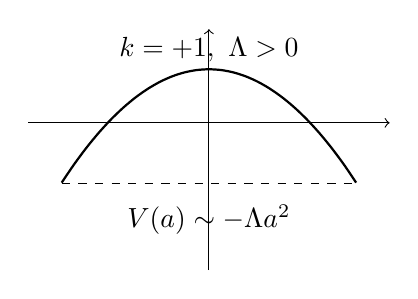
\begin{tikzpicture}[scale=0.85]
\draw[->] (-2.7,0) -- (2.7,0);
\draw[->] (0,-2.2) -- (0,1.4);
\draw[thick,domain=-2.2:2.2,smooth] plot (\x,{-0.35*(\x)^2 + 0.8});
\draw[dashed] (-2.2,-0.9) -- (2.2,-0.9);
\node at (0,-1.45) {\(V(a)\sim -\Lambda a^2\)};
\node at (0,1.1) {\(k=+1,\ \Lambda>0\)};
\end{tikzpicture}
\hspace{2em}
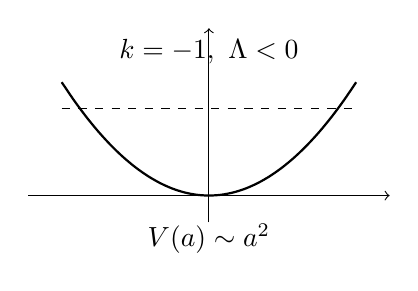
\begin{tikzpicture}[scale=0.85]
\draw[->] (-2.7,0) -- (2.7,0);
\draw[->] (0,-0.4) -- (0,2.5);
\draw[thick,domain=-2.2:2.2,smooth] plot (\x,{0.35*(\x)^2});
\draw[dashed] (-2.2,1.3) -- (2.2,1.3);
\node at (0,-0.65) {\(V(a)\sim a^2\)};
\node at (0,2.15) {\(k=-1,\ \Lambda<0\)};
\end{tikzpicture}
\caption{閉じたド・ジッター・バウンスと開いた負の \(\Lambda\) 再収縮に対する模式的な有効ポテンシャル。}
\label{fig:c05-mechanical-potentials}
\end{figure}

\begin{classroomqa}
\audiencequestion{これらのフリードマン方程式は本当にアインシュタイン方程式なのか？}
\lecturerresponse{はい。それらは、一様性と等方性が計量を単一の関数 \(a(t)\) に還元した後のアインシュタイン場の方程式である。対称性による還元はほとんどのテンソル成分を取り除き、宇宙膨張に対するこの常微分方程式を残す。\lecturetimestamp{01:43:52--01:44:05}}
\end{classroomqa}

\begin{classroomqa}
\audiencequestion{スケール因子 \(a\) は複素数になりうるか？}
\lecturerresponse{ここで解析している実の古典的 FRW 宇宙論ではそうではない。スケール因子は空間の大きさを測るものであり、実で非負とされる。複素化された幾何は他の数学的アプローチに現れうるが、この講義の解では役割をもたない。\lecturetimestamp{01:44:06--01:44:21}}
\end{classroomqa}

\begin{classroomqa}
\audiencequestion{圧力が密度の線形関数でなければならない物理的理由はあるか？}
\lecturerresponse{いいえ。一定の \(w\) は便利であり、たまたまここで考える主要な成分を記述する。物質、放射、真空の混合はすべての時代にわたって一つの一定な \(w\) をもつわけではなく、一般の物質は非線形な \(P(\rho)\) をもちうる。バロトロピック流体では、\(c=1\) とする単位で \(dP/d\rho\) が二乗音速を制御する；一定の \(w\) はその導関数を一定にするが、自然はそうする義務を負わない。\lecturetimestamp{01:44:21--01:45:34}}
\end{classroomqa}

\section{持ち越すべきこと}

状態方程式は微視的物理とスケール因子の時間履歴を結びつける。共動箱内の断熱仕事は
\[
\rho\propto a^{-3(1+w)}.
\]
を与える。冷たい物質は \(w=0\) と \(\rho\propto a^{-3}\) をもつ。等方な光子運動量流は
\[
\left\langle\cos^2\theta\right\rangle=\frac13,
\qquad
P_{\mathrm r}=\frac{\rho_{\mathrm r}}{3},
\qquad
\rho_{\mathrm r}\propto a^{-4}.
\]
を与える。

張力は負の圧力を物理的に理解可能にする。一定の真空密度は
\[
P_\Lambda=-\rho_\Lambda,
\qquad
w_\Lambda=-1.
\]
を満たす。正の真空エネルギーは平坦なスライシングで指数関数的なド・ジッター膨張を与え、閉じたスライシングで \(\cosh\) バウンスを与える。負の真空エネルギーは開いた宇宙さえも再収縮させうる。どの符号の場合でも、フリードマン方程式は有効な力学的エネルギー方程式として読むことができる。未解決の問題は、なぜ量子場が真空エネルギーに寄与するのかということではなく、なぜそれらの観測される正味の寄与がちょうどゼロではなくほとんどゼロなのかということである。
